
\section{Introduction}

Depression has been a major health challenge to the world, with over 280 million people affected, according to WHO\footnote{\url{https://www.who.int/news-room/fact-sheets/detail/depression}}. Moreover, the COVID-19 pandemic has further deteriorated the situation. The patients are more likely to suffer from depression due to poor health condition as well as perceived stigmatization. Since people are more willing to express their feelings on online social media during this special period\footnote{\url{https://www.statista.com/statistics/1106498/home-media-consumption-coronavirus-worldwide-by-country/}}, depression detection from online posts can be a promising approach to combat the challenge. The increasing difficulty for in-person clinical visits has also made such technique more vital than ever.

\begin{figure}[tbp]
    \centering
    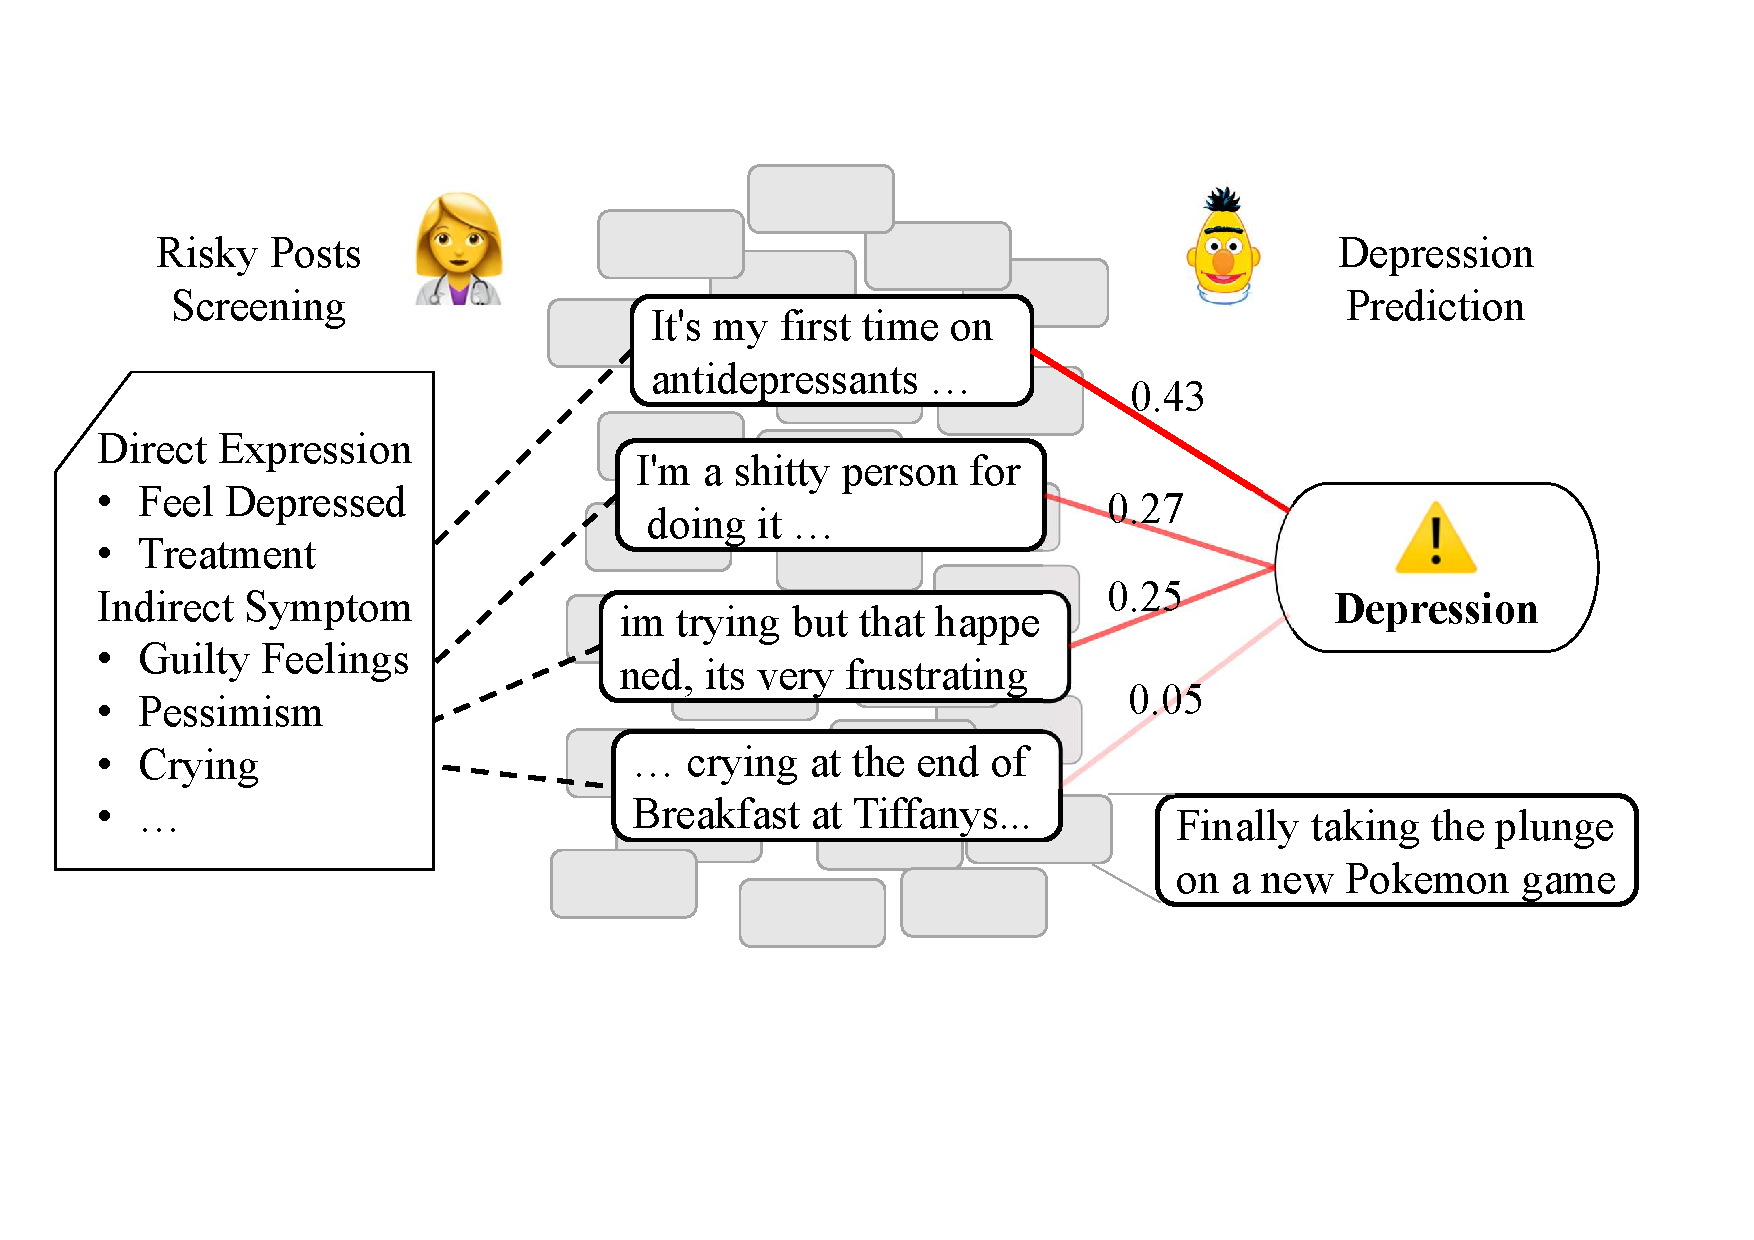
\includegraphics[width=\columnwidth]{figures/overview1.pdf}
    \caption{Overview of the system. Depression templates derived from established depression scales are used to screen risky posts, and filter out safer ones (boxes in grey). A hierarchical attentional network then further attends to truly important contents (transparency of the line indicates the attention strength) and makes final prediction. }
    % \KZ{Enlarge the fonts in the fig, and use a more legible font.}
    \label{fig:overview}
\end{figure}

Although remarkable progress has been made for automatic depression detection on social media \citep{trotzek2018utilizing, gui2019cooperative, zogan2021depressionnet}, several challenges still hinder the broad application of these techniques. First of all, most existing neural network-based methods for detecting depression lack explainability, despite a few pioneering works on post-level symptom identification \citep{mowery2017understanding}. Due to black box nature of NN models, we cannot confirm whether the model gives correct predictions by utilizing robust depression indicators, or some spurious clues. Specifically, their mechanism may not be intuitive enough for patients to understand, or 
consistent with the methodology in psychiatry. Without proper explanations, it can be hard for clinicians to trust such novel tools and for patients to accept these diagnosis results.

In addition, some studies have found that existing models do not generalize well 
in the presence of distribution gaps among online-collected depression 
datasets \citep{harrigian2020models}. For instance, within 3 datasets collected 
from Reddit \citep{losada2016test, yates2017depression, wolohan2018detecting}, 
there are differences in the included subreddits, the time span of the posting 
histories, and the approaches to annotate the depressed users. As is suggested by \citet{ernala2019methodological}, current mental health prediction models tend to overfit on the characteristics of a specific dataset instead of learning what they 
claim to measure (i.e., a robust disease indicator). Therefore, even if there exists similarities for attempts in domain adaptation, the performance of current models still tend to degrade significantly. This highlights the difficulty for existing models to learn generalizable features.

Finally, most previous works mainly focus on detecting depression from a person's entire post history, but overlook a more important and practical scenario, i.e.,
early detection~\citep{losada2017erisk}. Early depression detection aims to detect traces of depression as soon as possible. It has two aspects: Firstly, we hope to make accurate predictions as early as possible (i.e. when the user just posted a few posts). Secondly, the detection algorithm should be able to respond to each user post with a low time latency. This means that this algorithm is better to be an online, incremental algorithm that can update the prediction every time a user sends a post, rather than an offline batch algorithm that only runs once after a long interval. Neither of these two aspects can be handled easily, as is shown in the overview of eRisk2019, a competition of early risk detection, where most teams have to process the whole user posts, and resort to offline processing that takes several days \citep{losada2019overview}. 

Inspired by the psychiatry practice of using clinical scales to screen depression patients \citep{beck1996beck}, we propose to use depression templates derived from established depression scales to screen risky posts. These templates include direct expressions of depressive moods and depression treatments, as well as theory-grounding indirect symptoms like guilty feelings, pessimism and loss of appetite, etc. Only posts highly relevant to these templates will be selected out of the whole posting history, which can greatly reduce the number of posts, so as to eliminate distractors and improve processing efficiency. The psychiatry basis of the approach can also facilitate its generalizability. A hierarchical network incorporating attention mechanism \citep{yang2016hierarchical} and pretrained language model \citep{devlin2018bert} further aggregate the selected posts of a user, and assign higher weights to truly important contents for accurate and explainable predictions. The overview of our approach is illustrated in Figure \ref{fig:overview}. To enable early depression detection, we also propose an online algorithm based on a risky posts queue evolving with the streaming posts. Experimental results on 3 depression detection datasets show that our method can achieve state-of-the-art performance under in-domain settings, and also generalize better under cross-domain settings. With the proposed online algorithm, our method also demonstrates superior performance in early depression detection, and can be even faster than simple Logistic Regression models in processing all users' posts.

Our key contributions are as follows:
\begin{itemize}
    \item We propose psychiatry-guided risky post screening to select salient contents for processing, resulting in improved effectiveness, efficiency and generalizability.
    \item We utilize hierarchical attentional network with BERT (HAN-BERT) to make accurate and explainable predictions.
    \item We propose an online algorithm based on an evolving queue of risky posts to tackle the challenging task of early detection, achieving better performance in less time than competitive baselines. 
\end{itemize}
